\documentclass[a4paper,9pt]{extarticle}

%=========================================================
% PACKAGES
%=========================================================

\usepackage[
a4paper,
top=1.8cm,
bottom=1.5cm,
footskip=7mm,
left=1cm,
right=1cm,
headheight=14pt,
headsep=5mm
]{geometry}

\usepackage[T1]{fontenc}
\usepackage[utf8]{inputenc}
\usepackage[french]{babel}

\usepackage[sfdefault]{FiraSans}
\renewcommand{\familydefault}{\sfdefault}

\usepackage{multicol}
\setlength{\columnsep}{0.7cm}

\usepackage{amsmath,amssymb}
\usepackage{titlesec}
\usepackage{enumitem}

\usepackage{tcolorbox}
\tcbuselibrary{skins,breakable}

\usepackage{xcolor}
\usepackage{graphicx}
\usepackage{float}
\usepackage{tikz}

\usepackage{fancyhdr}
\usepackage[hidelinks]{hyperref}


%=========================================================
% PAGE SETTINGS
%=========================================================

\setlength{\parindent}{0pt}
\setlength{\parskip}{1.5pt}

\setlength{\abovedisplayskip}{4pt}
\setlength{\belowdisplayskip}{4pt}

\setlist[itemize]{
leftmargin=*,
itemsep=1pt,
topsep=1pt
}


%=========================================================
% COLORS
%=========================================================

\definecolor{Blue}{HTML}{E3F0FF}
\definecolor{Green}{HTML}{E3F7EA}
\definecolor{Pink}{HTML}{FFE5ED}
\definecolor{Orange}{HTML}{FFF0DC}
\definecolor{Purple}{HTML}{EEE7FF}
\definecolor{Yellow}{HTML}{FFFADB}

\definecolor{BlueTitle}{HTML}{285B8F}
\definecolor{GreenTitle}{HTML}{287052}
\definecolor{PinkTitle}{HTML}{A84063}
\definecolor{OrangeTitle}{HTML}{A96500}
\definecolor{PurpleTitle}{HTML}{6245A5}


%=========================================================
% HEADER
%=========================================================

\pagestyle{fancy}
\fancyhf{}

\fancyhead[L]{\small\textbf{Electronique I}}
\fancyhead[C]{\small Sources, Thévenin, Norton et superposition}
\fancyhead[R]{\small Week 04 -- 28/09-04/10/2026}

\fancyfoot[C]{\small\href{https://github.com/AlphaXT38G/notes_ba5}{github.com/AlphaXT38G/notes\_ba5}}
\fancyfoot[R]{\small \thepage}

\renewcommand{\headrulewidth}{0.4pt}


%=========================================================
% TITLES
%=========================================================

\titleformat{\section}
{\large\bfseries\color{BlueTitle}}
{}{0pt}{}

\titlespacing{\section}
{0pt}{6pt}{3pt}


%=========================================================
% SEPARATOR
%=========================================================

\newcommand{\separator}{
\vspace{2pt}
\hrule
\vspace{3pt}
}


%=========================================================
% BOXES
%=========================================================

% DEFINITION - blue

\newtcolorbox{definition}{
enhanced,
breakable,
colback=Blue,
colframe=BlueTitle,
boxrule=0.7pt,
arc=0mm,
title=\textbf{Definition},
fonttitle=\bfseries
}


% IMPORTANT - pink

\newtcolorbox{important}{
enhanced,
breakable,
colback=Pink,
colframe=PinkTitle,
boxrule=0.7pt,
arc=0mm,
title=\textbf{Key idea},
fonttitle=\bfseries
}


% FORMULAS - green

\newtcolorbox{formula}{
enhanced,
breakable,
colback=Green,
colframe=GreenTitle,
boxrule=0.7pt,
arc=0mm,
title=\textbf{Key formulas},
fonttitle=\bfseries
}


% WARNING - orange

\newtcolorbox{warning}{
enhanced,
breakable,
colback=Orange,
colframe=OrangeTitle,
boxrule=0.7pt,
arc=0mm,
title=\textbf{Warning},
fonttitle=\bfseries
}


% EXAMPLE - purple

\newtcolorbox{example}{
enhanced,
breakable,
colback=Purple,
colframe=PurpleTitle,
boxrule=0.7pt,
arc=0mm,
title=\textbf{Example},
fonttitle=\bfseries
}


% SUMMARY - yellow

\newtcolorbox{summary}{
enhanced,
breakable,
colback=Yellow,
colframe=OrangeTitle,
boxrule=0.7pt,
arc=0mm,
title=\textbf{Summary},
fonttitle=\bfseries
}


% a box only breaks once it has a few lines on this column: no lone title at the bottom
\tcbset{lines before break=8}


%=========================================================
% DOCUMENT
%=========================================================

\begin{document}

\thispagestyle{fancy}

\footnotesize

\begin{multicols}{2}


%=========================================================
\section{Dipôles actifs et passifs}


\begin{definition}

\textbf{Dipôle actif}

A une source d'énergie à l'intérieur : il a des sources actives.

\end{definition}


\begin{definition}

\textbf{Dipôle passif}

Il n'y a pas de source. Exemple : la résistance.

\end{definition}


%=========================================================
\section{Transformation de sources [1] : source linéaire de tension}


\begin{center}

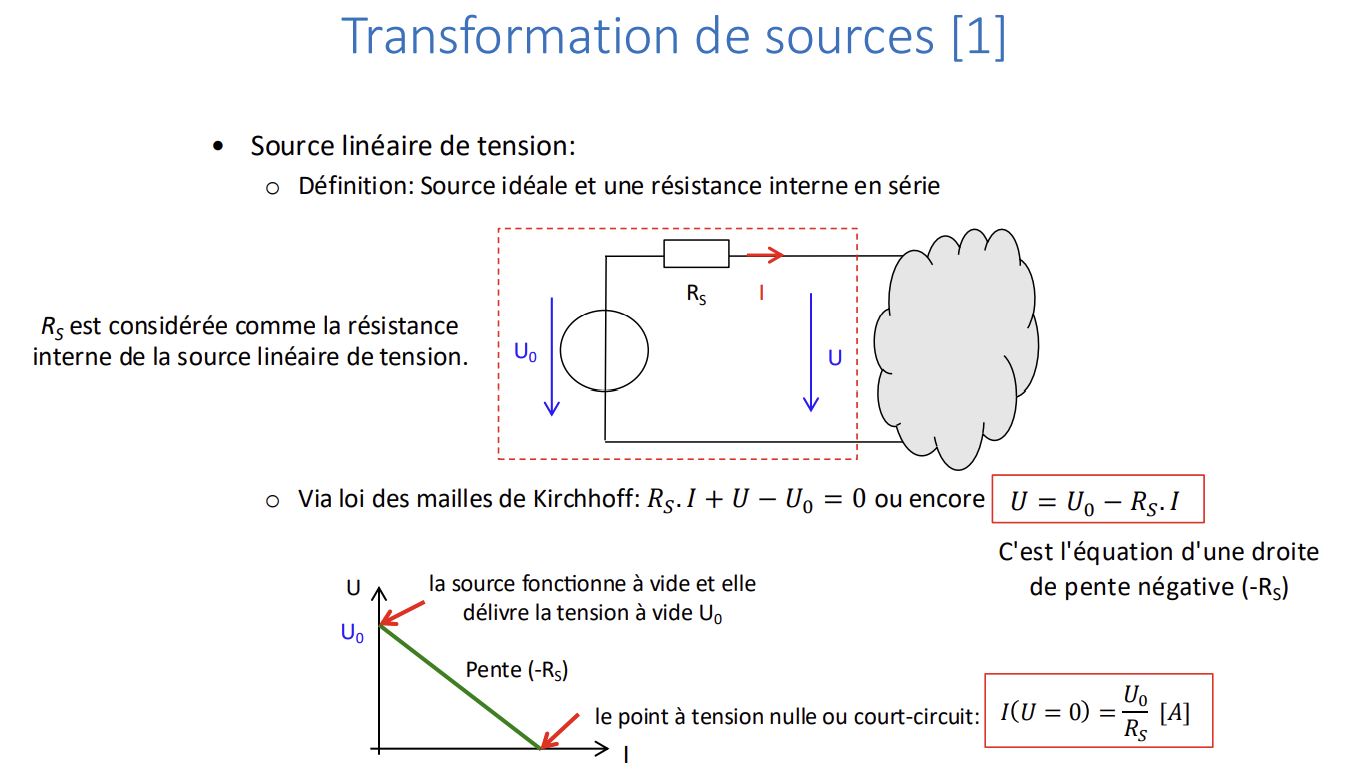
\includegraphics[
width=1.0\linewidth
]{../images/week04_01.png}

\end{center}


\begin{definition}

\textbf{Source linéaire de tension}

Source idéale et une résistance interne en série. $R_S$ est considérée comme la résistance interne de la source linéaire de tension.

\end{definition}


\begin{formula}

Via la loi des mailles de Kirchhoff :

\[
R_S\,I + U - U_0 = 0
\quad\text{ou encore}\quad
\boxed{U = U_0 - R_S\,I}
\]

C'est l'équation d'une droite de pente négative ($-R_S$).

\[
I(U = 0) = \frac{U_0}{R_S}\ [\text{A}]
\]

où :

\begin{itemize}

\item $U_0$ : tension de la source idéale = tension à vide [V] ;

\item $R_S$ : résistance interne (en série) [$\Omega$] ;

\item $I$ : courant débité vers l'extérieur (le \og nuage \fg{}) [A] ;

\item $U$ : tension disponible aux bornes de sortie [V] ;

\item $I(U=0)$ : courant de court-circuit [A].

\end{itemize}

\end{formula}


\begin{important}

\textbf{Le problème}

Une vraie pile n'est pas une source idéale : plus on lui demande de courant, plus sa tension baisse un peu. On la modélise donc par une source idéale $U_0$ \textbf{plus} une petite résistance $R_S$ cachée à l'intérieur.

\vspace{3pt}

\textbf{Ce qui se passe}

Le courant $I$ qui sort de la pile traverse d'abord $R_S$. Dans $R_S$, il \og perd \fg{} une tension $R_S\,I$ (loi d'Ohm). Ce qui reste pour l'extérieur, c'est $U = U_0 - R_S\,I$ : plus $I$ est grand, plus on perd.

\vspace{3pt}

\textbf{Lire le graphe (une droite qui descend)}

\begin{itemize}

\item \textbf{À vide} (rien de branché, $I = 0$) : rien ne se perd dans $R_S$, donc $U = U_0$. C'est le point en haut, sur l'axe $U$.

\item \textbf{Court-circuit} (un fil entre les bornes, $U = 0$) : toute la tension $U_0$ est perdue dans $R_S$, et le courant est le plus grand possible, $I = U_0/R_S$. C'est le point en bas, sur l'axe $I$.

\item Entre les deux, la droite descend avec la pente $-R_S$ : chaque ampère en plus fait perdre $R_S$ volts.

\end{itemize}

\end{important}


\begin{example}

Pile $U_0 = 9\,\text{V}$, $R_S = 1\,\Omega$ :

\begin{itemize}

\item à vide : $U = 9\,\text{V}$ ;

\item elle débite $I = 1\,\text{A}$ : $U = 9 - 1\cdot 1 = 8\,\text{V}$ ;

\item en court-circuit : $I = 9/1 = 9\,\text{A}$ et $U = 0\,\text{V}$.

\end{itemize}

\end{example}


%=========================================================
\section{Transformation de sources [2] : source linéaire de courant}


\begin{center}

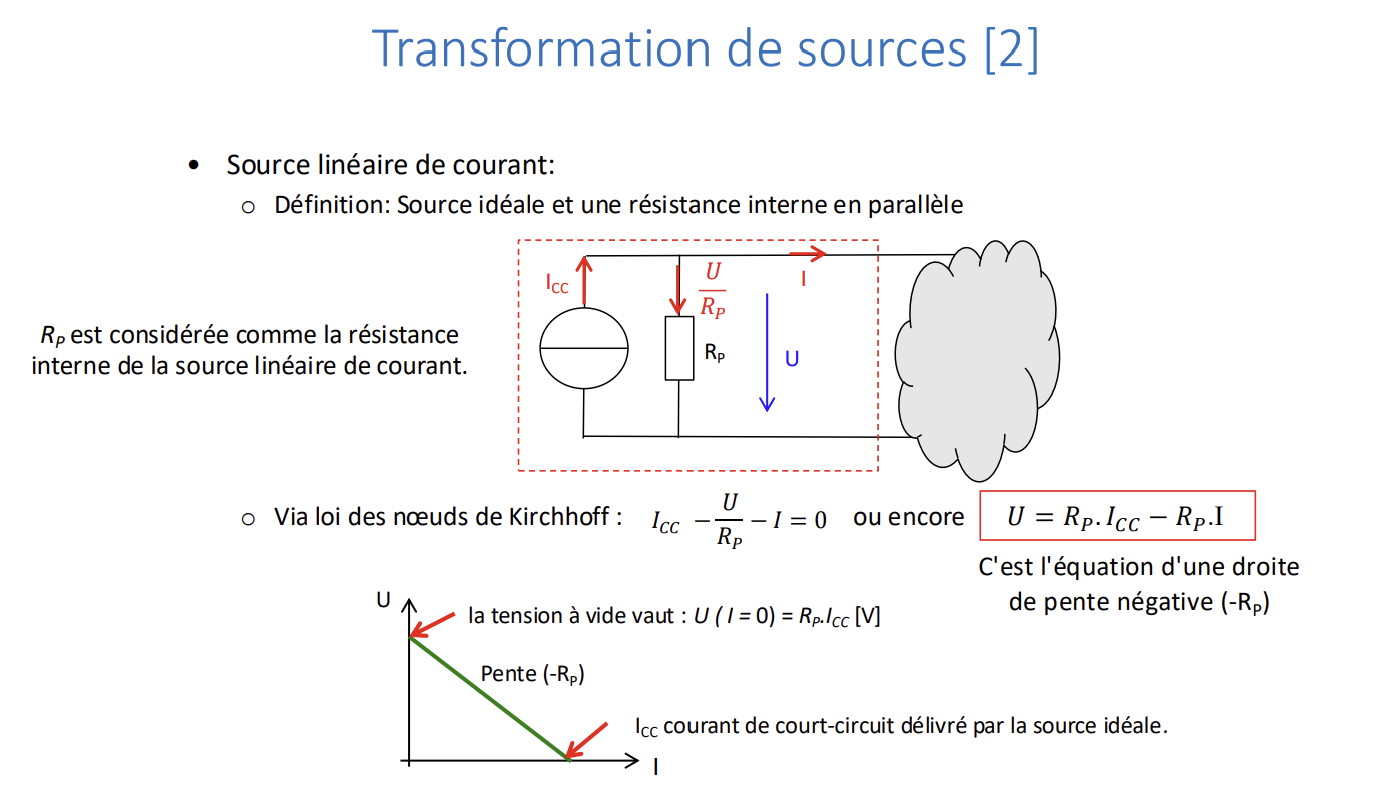
\includegraphics[
width=1.0\linewidth
]{../images/week04_02.png}

\end{center}


\begin{definition}

\textbf{Source linéaire de courant}

Source idéale et une résistance interne en parallèle. $R_P$ est considérée comme la résistance interne de la source linéaire de courant.

\end{definition}


\begin{formula}

Via la loi des nœuds de Kirchhoff :

\[
I_{CC} - \frac{U}{R_P} - I = 0
\quad\text{ou encore}\quad
\boxed{U = R_P\,I_{CC} - R_P\,I}
\]

C'est l'équation d'une droite de pente négative ($-R_P$).

\[
U(I = 0) = R_P\,I_{CC}\ [\text{V}]
\]

où :

\begin{itemize}

\item $I_{CC}$ : courant de la source idéale = courant de court-circuit [A] ;

\item $R_P$ : résistance interne (en parallèle) [$\Omega$] ;

\item $U/R_P$ : courant qui part dans $R_P$ [A] ;

\item $I$ : courant débité vers l'extérieur [A] ;

\item $U$ : tension aux bornes de sortie [V] ;

\item $U(I=0)$ : tension à vide [V].

\end{itemize}

\end{formula}


\begin{important}

\textbf{L'image}

La source idéale pousse toujours le même débit $I_{CC}$, comme une pompe. Mais à côté de la sortie, il y a une \og fuite \fg{} : la résistance $R_P$ en parallèle. Le courant se partage : une partie $U/R_P$ part dans la fuite, le reste $I$ va vers l'extérieur.

\vspace{3pt}

\textbf{Lire le graphe (encore une droite qui descend)}

\begin{itemize}

\item \textbf{À vide} (rien de branché, $I = 0$) : tout le courant part dans la fuite $R_P$, qui a donc la tension $U = R_P\,I_{CC}$ à ses bornes. C'est le point en haut.

\item \textbf{Court-circuit} (un fil entre les bornes, $U = 0$) : le fil est bien plus facile que $R_P$, donc plus rien ne passe dans la fuite ($U/R_P = 0$) : tout sort, $I = I_{CC}$. C'est le point en bas.

\item Entre les deux, la pente vaut $-R_P$.

\end{itemize}

\vspace{3pt}

\textbf{À retenir :} même forme de graphe que la source de tension. C'est ce qui permet de passer de l'une à l'autre (section suivante).

\end{important}


\begin{example}

$I_{CC} = 9\,\text{A}$, $R_P = 1\,\Omega$ :

\begin{itemize}

\item à vide : $U = 1 \cdot 9 = 9\,\text{V}$ ;

\item elle débite $I = 1\,\text{A}$ : $U = 9 - 1\cdot 1 = 8\,\text{V}$ ;

\item en court-circuit : $I = 9\,\text{A}$ et $U = 0\,\text{V}$.

\end{itemize}

Exactement les mêmes chiffres que la pile de l'exemple précédent !

\end{example}


%=========================================================
\section{Transformation de sources [3] : tension $\leftrightarrow$ courant}


\begin{center}

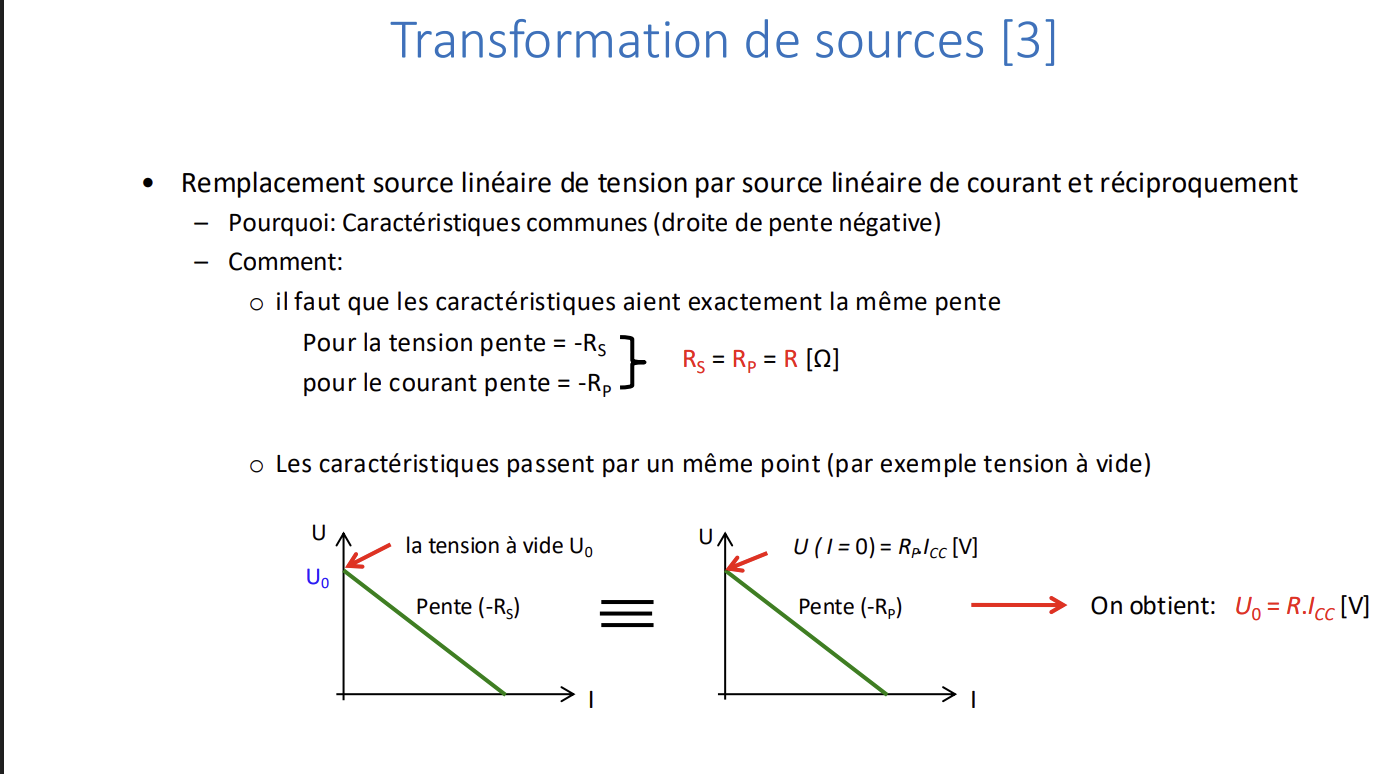
\includegraphics[
width=1.0\linewidth
]{../images/week04_03.png}

\end{center}


\textbf{Remplacement d'une source linéaire de tension par une source linéaire de courant, et réciproquement.}

\begin{itemize}

\item \textbf{Pourquoi :} caractéristiques communes (droite de pente négative).

\item \textbf{Comment :} il faut que les caractéristiques aient exactement la même pente, et qu'elles passent par un même point (par exemple la tension à vide).

\end{itemize}


\begin{formula}

Même pente : pour la tension, pente $= -R_S$ ; pour le courant, pente $= -R_P$ :

\[
R_S = R_P = R\ [\Omega]
\]

Même point (tension à vide) : $U_0$ d'un côté, $U(I=0) = R_P\,I_{CC}$ de l'autre. On obtient :

\[
\boxed{U_0 = R\,I_{CC}}\ [\text{V}]
\]

où :

\begin{itemize}

\item $R$ : la résistance interne commune [$\Omega$] (en série pour la source de tension, en parallèle pour la source de courant) ;

\item $U_0$ : tension de la source de tension [V] ;

\item $I_{CC}$ : courant de la source de courant [A].

\end{itemize}

\end{formula}


\begin{important}

\textbf{L'idée}

Imagine deux boîtes fermées avec deux fils qui sortent. Dans l'une, une source de tension avec une résistance en série ; dans l'autre, une source de courant avec une résistance en parallèle. Si, quoi qu'on branche dessus, elles donnent toujours la même tension et le même courant, alors de l'extérieur il est \textbf{impossible} de savoir laquelle est laquelle : on peut remplacer l'une par l'autre.

\vspace{3pt}

\textbf{Comment s'en assurer}

Ce que donne une boîte, c'est sa droite $U(I)$. Deux droites sont identiques si elles ont la même pente \textbf{et} un point en commun :

\begin{enumerate}[leftmargin=*,itemsep=1pt,topsep=1pt]

\item même pente $\Rightarrow$ même résistance $R$ des deux côtés ;

\item même tension à vide $\Rightarrow$ $U_0 = R\,I_{CC}$.

\end{enumerate}

\textbf{La recette}

\begin{itemize}

\item Tension $\to$ courant : on garde $R$ (on la met en parallèle) et on prend $I_{CC} = U_0/R$.

\item Courant $\to$ tension : on garde $R$ (on la met en série) et on prend $U_0 = R\,I_{CC}$.

\end{itemize}

\textbf{À quoi ça sert}

À simplifier : des sources de courant en parallèle s'additionnent, des sources de tension en série aussi. On transforme pour se retrouver dans le cas facile.

\end{important}


\begin{example}

\textbf{Pile $9\,\text{V}$ et $1\,\Omega$ en série} $\Leftrightarrow$ \textbf{source de $9\,\text{A}$ avec $1\,\Omega$ en parallèle} ($I_{CC} = 9/1$).

\vspace{3pt}

Vérification avec une charge de $8\,\Omega$ branchée dessus :

\begin{itemize}

\item version tension : $I = \frac{9}{1 + 8} = 1\,\text{A}$, donc $U = 8 \cdot 1 = 8\,\text{V}$ ;

\item version courant : les $9\,\text{A}$ se partagent entre $1\,\Omega$ et $8\,\Omega$ ; dans la charge, $I = 9\cdot\frac{1}{1 + 8} = 1\,\text{A}$, donc $U = 8\,\text{V}$.

\end{itemize}

Même résultat : la charge ne voit aucune différence.

\end{example}


\end{multicols}

\end{document}
